% ****** Start of file apssamp.tex ******
%
%   This file is part of the APS files in the REVTeX 4.2 distribution.
%   Version 4.2a of REVTeX, December 2014
%
%   Copyright (c) 2014 The American Physical Society.
%
%   See the REVTeX 4 README file for restrictions and more information.
%
% TeX'ing this file requires that you have AMS-LaTeX 2.0 installed
% as well as the rest of the prerequisites for REVTeX 4.2
%
% See the REVTeX 4 README file
% It also requires running BibTeX. The commands are as follows:
%
%  1)  latex apssamp.tex
%  2)  bibtex apssamp
%  3)  latex apssamp.tex
%  4)  latex apssamp.tex
%
\documentclass[%
 reprint,
%superscriptaddress,
%groupedaddress,
%unsortedaddress,
%runinaddress,
%frontmatterverbose, 
%preprint,
%preprintnumbers,
%nofootinbib,
%nobibnotes,
%bibnotes,
 amsmath,amssymb,
 aps,
%pra,
%prb,
%rmp,
%prstab,
%prstper,
%floatfix,
]{revtex4-2}
\usepackage{kotex}
\usepackage{graphicx}% Include figure files
\usepackage{dcolumn}% Align table columns on decimal point
\usepackage{bm}% bold math
%\usepackage{hyperref}% add hypertext capabilities
%\usepackage[mathlines]{lineno}% Enable numbering of text and display math
%\linenumbers\relax % Commence numbering lines

%\usepackage[showframe,%Uncomment any one of the following lines to test 
%%scale=0.7, marginratio={1:1, 2:3}, ignoreall,% default settings
%%text={7in,10in},centering,
%%margin=1.5in,
%%total={6.5in,8.75in}, top=1.2in, left=0.9in, includefoot,
%%height=10in,a5paper,hmargin={3cm,0.8in},
%]{geometry}

\def\rcurs{{\mbox{$\resizebox{.16in}{.08in}{
\includegraphics{ScriptR}}$}}}
\def\brcurs{{\mbox{$\resizebox{.16in}{.08in}{
\includegraphics{BoldR}}$}}}
\def\hrcurs{{\mbox{$\hat \brcurs$}}}

\begin{document}


\title{약산의 적정과 분리 실험 결과보고서}

\author{서울대학교 전기정보공학부 2018-12432 박정현}
 \email{alexist@snu.ac.kr}
\date{실험 일자 09.19.2023, 제출일자 09.24.2023}% It is always \today, today,
\author{담당 조교님: 김지윤 조교님}
\author{담당 교수님: David Yu-Kai Chen}
             %  but any date may be explicitly specified

\begin{abstract}
본 실험에서는 산염기 적정을 이용해 미지의 물질의 농도를 측정하고 역상크로마토그래피를 이용해 극성에 따라 물질을 분리하여 각각의 몰농도를 측정한다. 이를통해 산염기 반응에 대한 이해도와 크로마토그래피에서 극성에 따른 이동상, 정지상의 역할을 이해한다. 실험 결과에서 sharp, braod한 이유와 기타 오차가 발생한 이유를 논하였다.
\end{abstract}

%\keywords{Suggested keywords}%Use showkeys class option if keyword
                              %display desired
\maketitle

%\tableofcontents

\section{\label{sec:level1}Assignment}
\subsection{\label{sec:level2}Problem1}
약산을 $HA$이라고 가정하자. 이때 $NaOH$와의 반응은 아래와 같다. 이 때 아래의 식이 성립한다.
\begin{align}
	HA(aq) + NaOH(aq) \rightarrow Na^{+}(aq) + A^{-}(aq) + H_{2}O(l)
\end{align}

\begin{align}
	K_{a} &= \frac{([H^{+}][A^{-}]}{[HA]}\\
\end{align}
식을 정리하면 아래와 같은 Henderson-Hasselbalch 식으로 정리된다.[3]
\begin{align}
	pH &= pK_{a} + \log \frac{[A^{-}]}{[HA]}
\end{align}
$NaOH$는 강산이므로 투입한 $NaOH$만큼 반응할 것이고반 당량점에서는  $[HA] = [A^{-}]$가 성립하므로 $pH = pK_{a} = 4.85$이다. 따라서 이온화 상수는 아래와 같다.
\begin{align}
	K_{a} &= 10^{-4.85}[mol/L]\\
	&=1.41 \times 10^{-5}[mol/L]
\end{align}
당량점에서 대해서 아래의 식이 성립한다.
\begin{align}
	n_{HA}V_{HA}M_{HA} = n_{NaOH}V_{NaOH}M_{NaOH}
\end{align}
각각의 경우 모두 하나의 작용기가 반응하므로 $n=1$이다. 따라서 약산의 농도는 아래와 같다.
\begin{align}
	M_{HA} &= \frac{V_{NaOH}M_{NaOH}}{V_{HA}}\\
	&=\frac{39.30mL \times 0.1000mol/L}{50.00mL}\\
	&= 0.07860 [mol/L]
\end{align}
\subsection{\label{sec:level2}Problem2}
아세트산, 살리실산과 아스피린(아세틸 살리실산)의 분자구조는 각각 Fig.\ref{fig:acet}[2], \ref{fig:saly}[3] , \ref{fig:aspirin}[2]와 같다. 아세트산의 경우 $COOH$가 극성을 띠고 분자 크기중 절반 가량이 아세틸기가 차지하므로 가장 강한 극성을 띨 것이다. 살리실산의 경우 카복실기와 하이드록시기를 가지지만 분자의 대부분이 페닐기로 구성되어 약한 극성을 나타낸다. 반면에 아스피린의 경우 카복실기와 메틸에스터기를 가지고 있다. 아스피린의 극성 뿐만 아니라 메틸에스터기의 산소 원자들의 비공야 전자쌍들이 강한 극성을 만들고 크기또한 분자의 크기에서 절반가까이 점유하고 있기 때문에 살리실산보다는 더 큰 극성을 띨 것이다. 하지만 아세트산보다 분자에서 극성을 만드는 부분의 크기가 작으므로 아세트산보다는 작은 극성을 띨 것이다. C18카트리지에서 이동상은 극성, 정지상은 비극성 분자에 해당하므로 아세트산, 아스피린, 살리실산 순서로 물질이 나오게 된다.

\begin{figure}[htbp]
	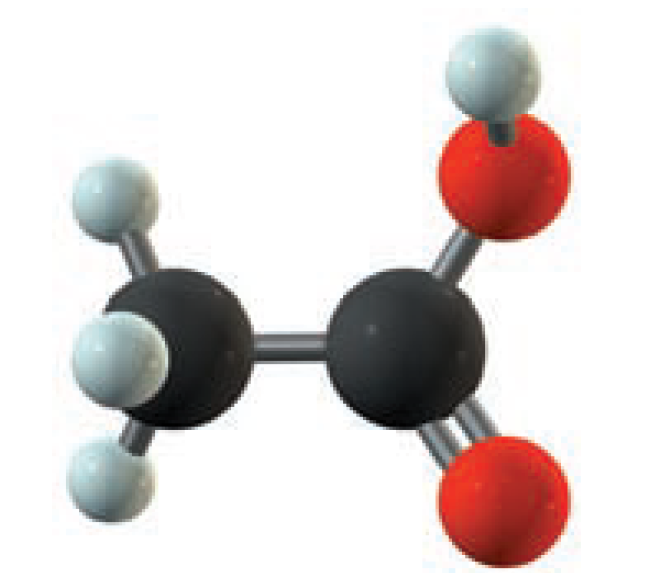
\includegraphics[width = 0.5\linewidth]{acet.png}% Here is how to import EPS art
	\caption{\label{fig:acet}아세트산 분자구조}
\end{figure}
\begin{figure}[htbp]
	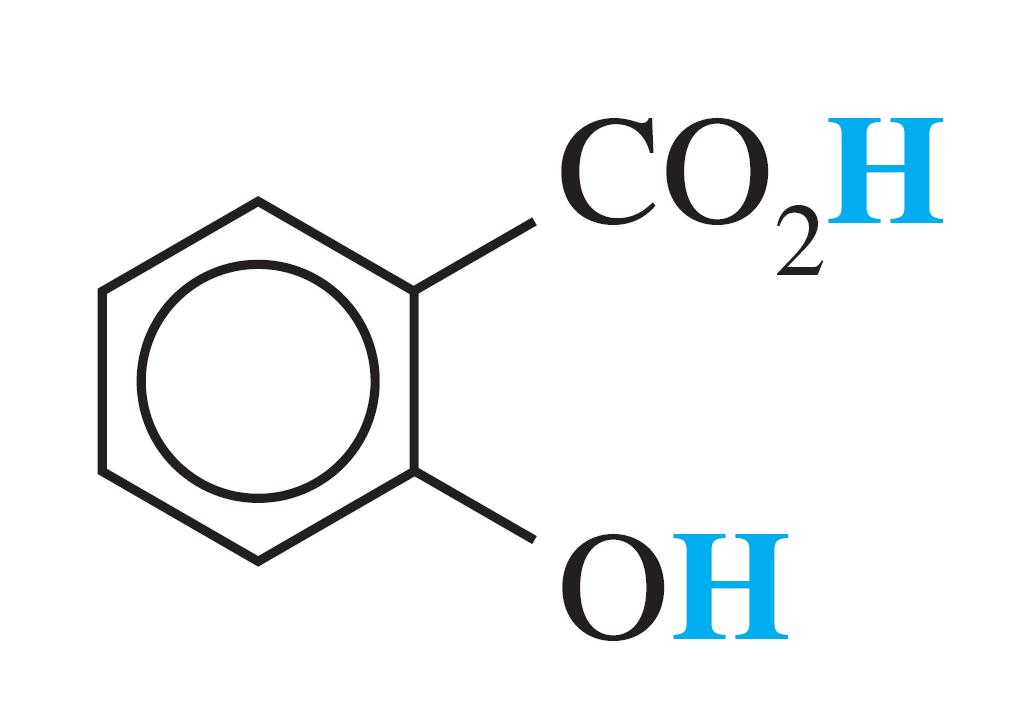
\includegraphics[width = 0.5\linewidth]{saly.png}% Here is how to import EPS art
	\caption{\label{fig:saly}살리실산 분자구조}
\end{figure}
\begin{figure}[htbp]
	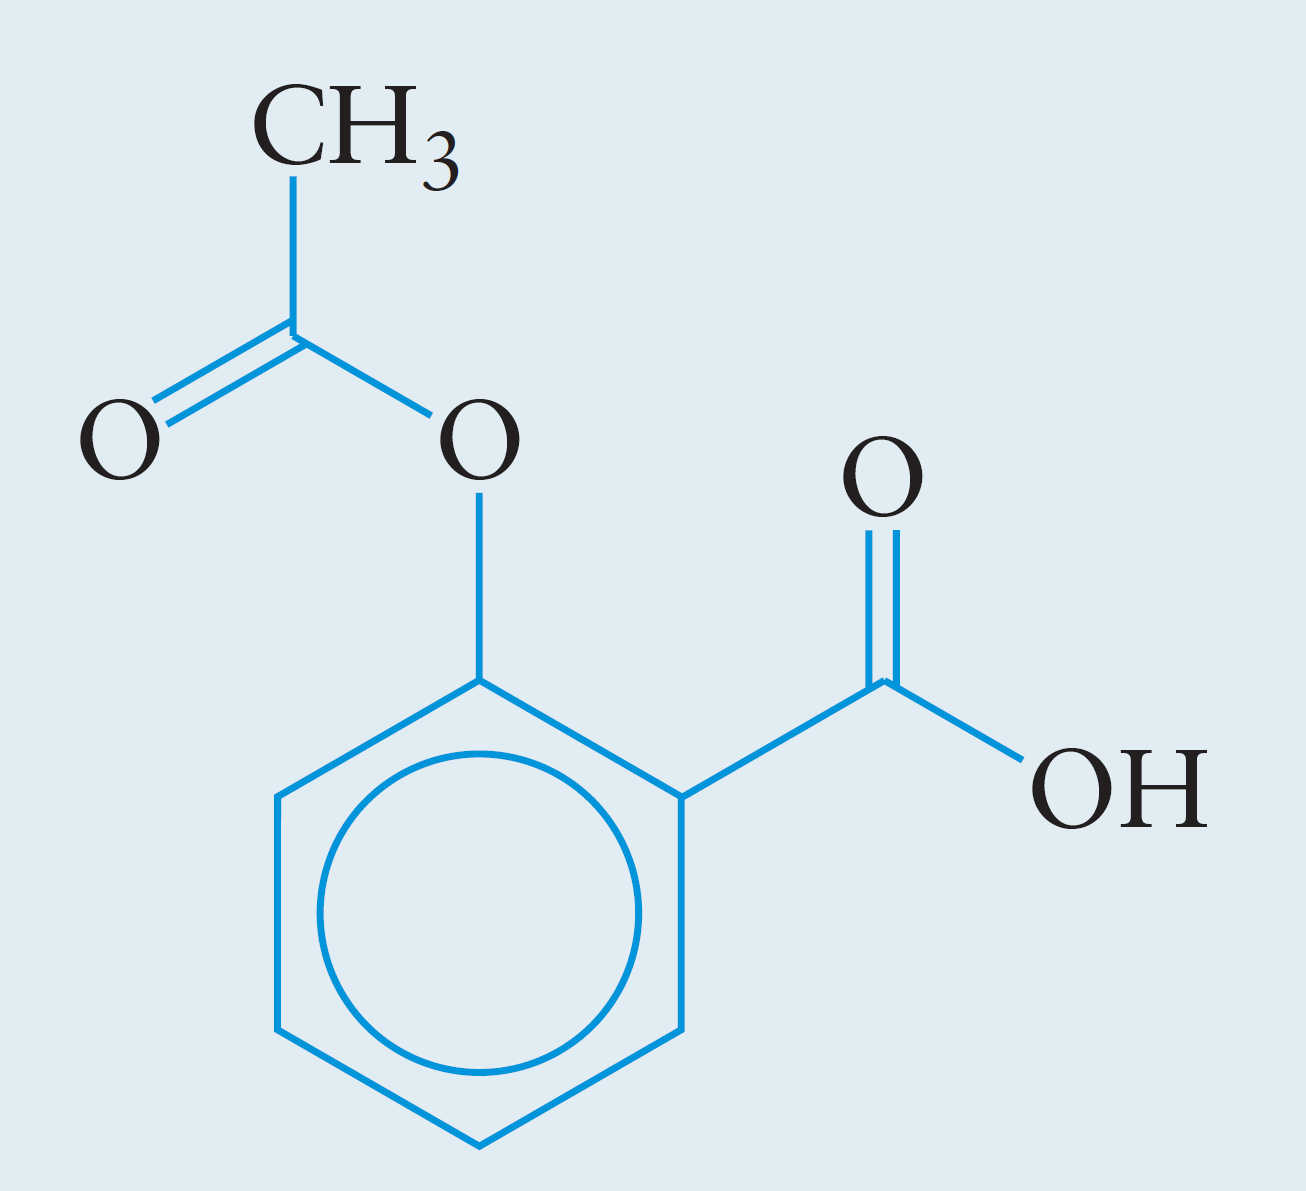
\includegraphics[width = 0.5\linewidth]{aspirin.png}% Here is how to import EPS art
	\caption{\label{fig:aspirin}아스피린 분자구조}
\end{figure}

또한 이온 교환 방식의 크로마토그래피에서 동일한 결과를 확인할 수 있다.[4] 해당 크로마토그래피에서도 극성이 강할 경우 더 빠르게 이동하게 되므로 C18 카트리지를 이용한 크로마토그래피와 동일한 결과를 보일 것을 예상할 수 있다. Fig.\ref{fig:EXP_P}는 해당 실험 결과이다.

\begin{figure}[htbp]
	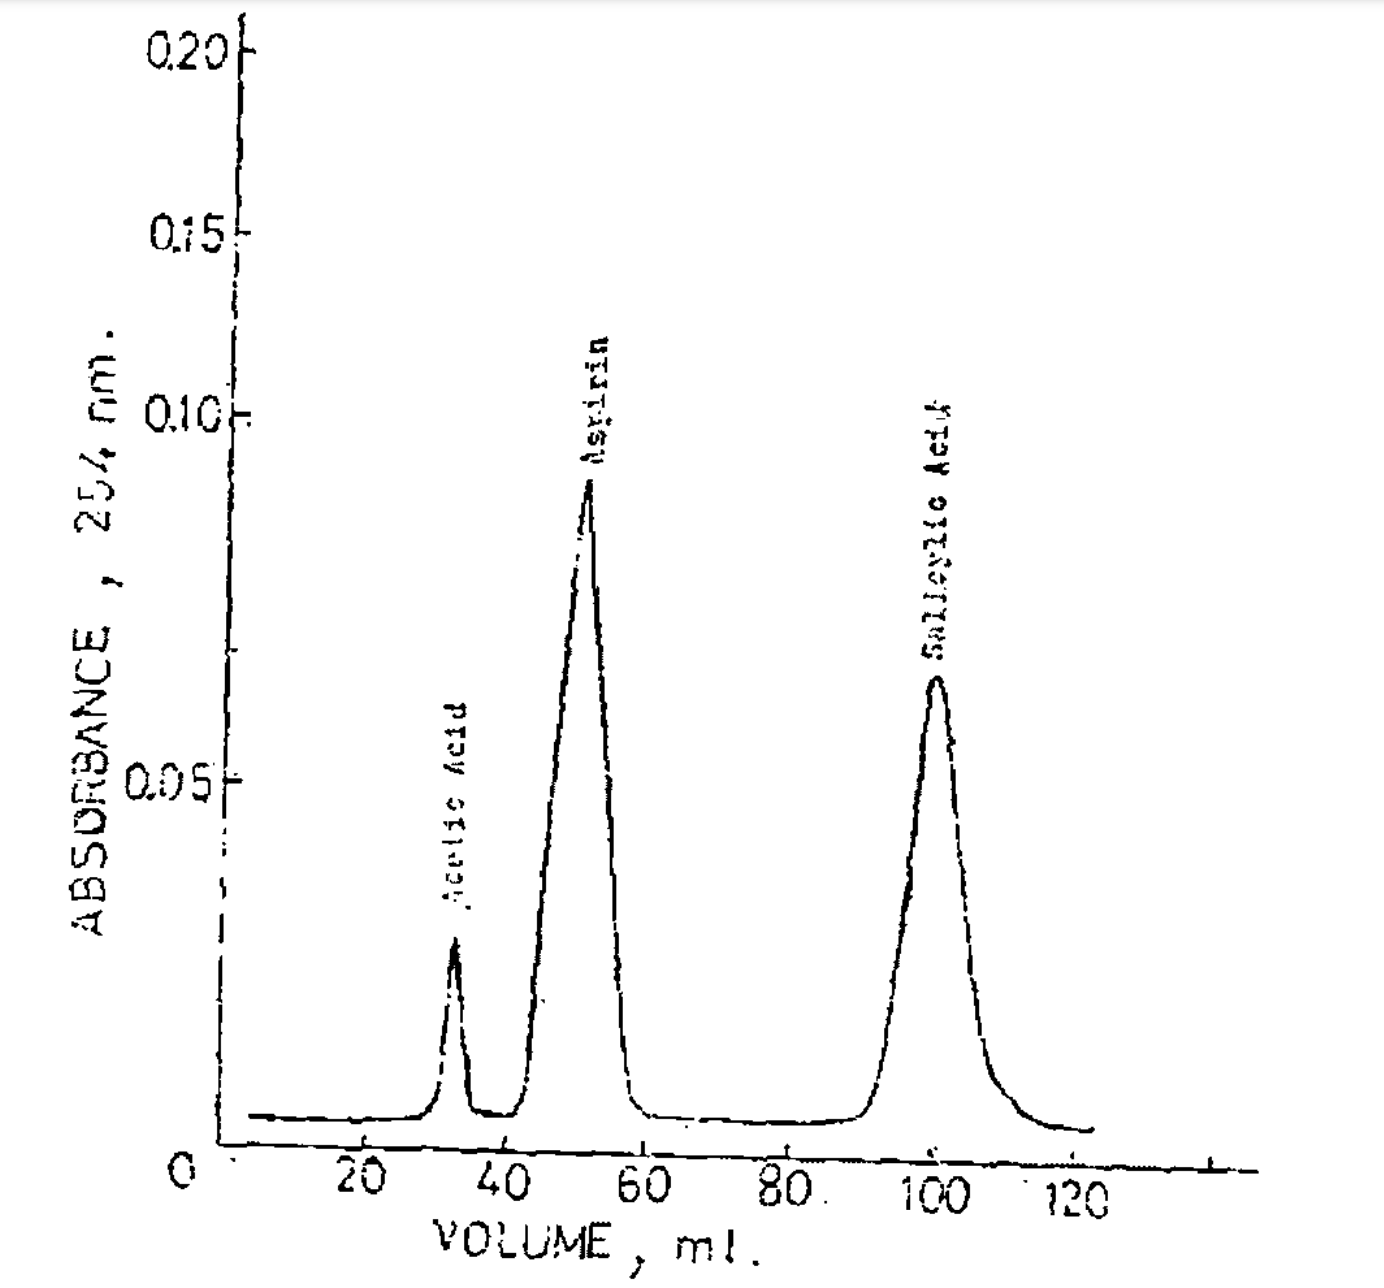
\includegraphics[width = 0.9\linewidth]{EXP_P.png}% Here is how to import EPS art
	\caption{\label{fig:EXP_P}아세트산, 아스피린, 살리실산 분리실}
\end{figure}

\section{\label{sec:level1}Introduction}
\subsection{\label{sec:level2}$NaOH$표준화}
$KHP$와 $NaOH$ 화학 반응식은 아래와 같다.
\begin{align}
	NaOH + KHC_{8}H_{4}O_{4} &\rightarrow KNaC_{8}H_{4}O_{4} + H_{2}O
\end{align}
본 실험에서 사용된 표준 용액은 $KHC_{8}H_{4}O_{4}$ $6mM$이다. 이 때 당량점에서 아래의 식이 성립한다. 이 때 위의 반응식에서 각각 하나의 $H^{+}$, $OH^{-}$가 반응하게 되므로 $n_{KHP}$, $n_{NaOH}$의 값은 $1$이다.
\begin{align}
	n_{KHP}M_{KHP}V_{KHP} &= n_{NaOH}M_{NaOH}V_{NaOH}\\
	V_{NaOH} &= \frac{M_{KHP}V_{KHP}}{M_{NaOH}}
\end{align}
이때 증류수 바탕적정에 투입된 $NaOH$의 양을 뺀 뒤 사용된 위의 식을 이용해 $NaOH$의 농도를 계산할 수 있다.


\subsection{\label{sec:level2}약산의 total acidity}
$CH_{3}(COOH)$, ($C_{6}H_{4}(OH)COOH$) 은 각 $pK_{a}=4.75$ [2], $pK_{a}=2.972$ [3]의 $pK_{a}$값을 가지며 $NaOH(aq)$와의 반응은 아래와 같다.

\begin{align}
	C_{7}H_{6}O_{3}(aq) \rightarrow C_{7}H_{5}O_{3}^{-}(aq) + H^{+}(aq) & pK_{a}=2.972\\
	C_{2}H_{4}O_{2}(aq) \rightarrow C_{2}H_{3}O_{2}^{-}(aq) + H^{+}(aq) & pK_{a}=4.75
\end{align}

따라서 total acidity에 대해서 아래의 식이 성립한다. 단, $M_{H^{+}}$는 약산이 모두 반응하는 총 몰수를 부피로 나눈 몰농도이다.

\begin{align}
	M_{H^{+}}V_{acid} &= V_{NaOH}M_{NaOH} \label{eq:total_acid}
\end{align}

\section{\label{sec:level1}Data and Results}
\subsection{\label{sec:level2}$NaOH$표준화}
$KHP$용액을 적정한 결과는 아래와 같다. 단, Tab.\ref{tab:NaOH_KHP}에서 오차는 최소 눈금으로 인한 오차이다. 해당 데이터를 선형회귀하면 Fig.\ref{fig:NaOH_KHP}와 같다.
\begin{table}[]
\begin{tabular}{c|c} \hline \hline
$KHP$ 부피[$mL$] & $NaOH$ 부피[$mL$] \\ \hline
$0.1\pm0.01$ & $3.38 - 3.18 - 0.04 = 0.16\pm0.02$  \\ \hline
$0.5\pm0.01$ & $4.30 - 3.50 - 0.04 = 0.76\pm0.02$  \\ \hline
$0.5\pm0.01$ & $5.11-4.35 - 0.04 = 0.72\pm0.02$ \\  \hline \hline 
\end{tabular}
\caption{\label{tab:NaOH_KHP}측정된 화학 반응여부}
\end{table}

\begin{figure}[htbp]
	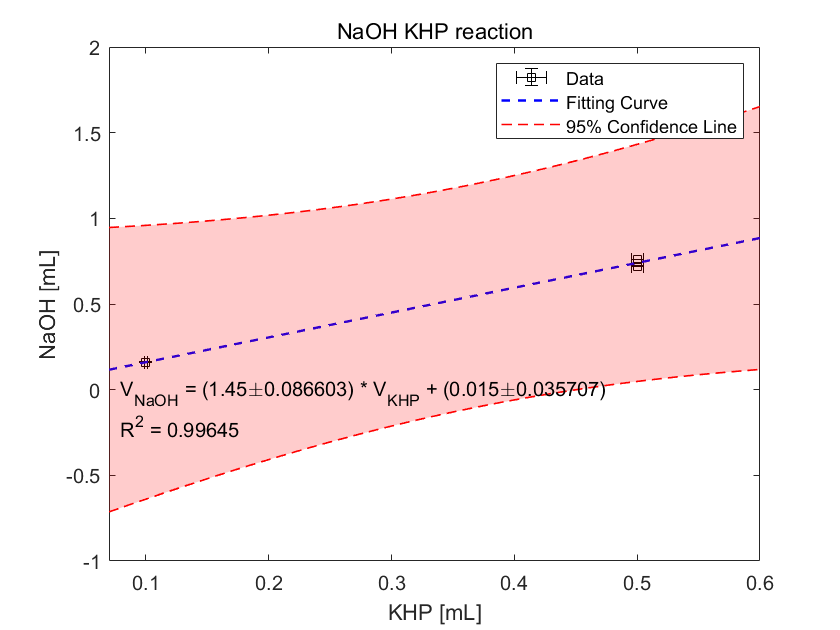
\includegraphics[width = 0.95\linewidth]{NaOH_KHP.png}% Here is how to import EPS art
	\caption{\label{fig:NaOH_KHP}$NaOH$, $KHP$ 반응부피에 대한 그래프}
\end{figure}
그래프의 기울기를 이용해 $NaOH$의 몰수를 계산하면 아래와 같다. 이 때 오차는 선형회귀 결과의 분산을 이용해 계산하였다.
\begin{align}
	M_{NaOH} &= 4.14 \pm 0.24 [mM]
\end{align}


\subsection{\label{sec:level2}약산의 total acidity}
약산의 혼합용액 $0.10mL$에 대해서 반응한 $NaOH$ 용액의 부피는 아래와 같다. 식 (\ref{eq:total_acid})을 이용했을 때 total acid는 아래와 같다. 단, 각각의 경우는 $NaOH$의 농도를 $1mM$로 둔 경우와 실제 측정된 $4.14mM$의 경우에 대해 계산한 결과이다. 그리고 $0.1mL$의 약산 용액을 적정한 경우와 비교하여 $1.0mL$의 약산 용액을 적정한 경우 $10$배를 곱해야한다.
\begin{align}
	V_{NaOH} &= (9.81 - 8.89 -0.04) = 0.88 \pm 0.01 [mL]
\end{align}

\begin{table}[]
\begin{tabular}{c|c} \hline \hline
$M_{NaOH} = 1mM$ & $M_{NaOH} = 4.14mM$ \\ \hline
$8.8\pm0.01mmol$ & $36.4\pm0.04mmol$  \\ \hline \hline
\end{tabular}
\caption{\label{tab:total acid}약산용액이 $1.0mL$일 때의 Total Acid}
\end{table}


\subsection{\label{sec:level2}약산의 분리}
C18카트리지를 $1mL$씩 밀며 적정했을 때 반응한 $NaOH$의 부피는 아래와 같다. 이를 그래프로 나타내면 Fig.\ref{fig:C18}와 같아진다. 총 반응부피는 $V_{total} = 6.74mL$에 해당한다. 이 때 가장 처음피크 부근의 총 반응부피는 $V_{first peak}$ $=6.17mL$이다. 이동상이 극성에 해당하므로 먼저 나온 물질은 아세트산, 그리고 나중에 나온 물질은 살리실산임을 알 수 있다. 당량점에서 $nMV = n'V'M'$이 성립하고 $0.1mL$의 약산이 반응한 부피가 $V_{NaOH}$ $=0.88mL$이므로 C18 카트리지와 잘 결합하는 분자와 잘 결합하지 않는 분자들의 몰 비율은 $(8.8 - 6.17):6.17=2.6:6.2$이다. 이 때 C18 카트리지의 경우 무극성 분자와 잘 결합하고 무극성 분자는 살리실산, 극성 분자는 아세트산이므로 살리실산과 아세트산의 비율이 $2.6:6.2$임을 알 수 있다. 따라서 각각의 총 몰수는 Tab.\ref{tab:NAOH_1}, \ref{tab:NAOH_4}와 같다. 
\begin{table}[]
\begin{tabular}{c|c} \hline \hline
이동 부피$\pm 0.01 [mL]$ & 반응한 $V_{NaOH} \pm0.01 [mL]$ \\ \hline
1 & $10.75-10.61  - 0.04 = 0.10$\\ \hline
2 & $14.82-10.75 - 0.04 = 4.03$\\ \hline
3 & $16.48-14.82 - 0.04 = 1.62$\\ \hline
4 &$ 16.88-16.48 - 0.04 = 0.36$\\ \hline
5 &$ 17.00-16.90 - 0.04 = 0.06$\\ \hline
6 &$ 17.05-17.00 - 0.04 = 0.01$\\ \hline
7 &$ 17.15-17.05 - 0.04 = 0.06$\\ \hline
8 &$ 17.30-17.15 - 0.04 = 0.11$\\ \hline
9 &$ 17.40-17.30 - 0.04 = 0.06$\\ \hline
10 &$ 17.50-17.40 - 0.04 = 0.06$\\ \hline
11 &$ 17.60-17.50 - 0.04 = 0.06$\\ \hline
12 &$ 17.65-17.60 - 0.04 = 0.01$\\ \hline
13 &$ 17.72-17.65 - 0.04 = 0.03$\\ \hline
14 &$ 17.80-17.72 - 0.04 = 0.04$\\ \hline
15 &$ 17.85-17.80 - 0.04 = 0.01$\\ \hline
16 &$ 17.92-17.85 - 0.04 = 0.03$\\ \hline
17 &$ 18.10-18.00 - 0.04 = 0.06$\\ \hline
18 &$ 18.12-18.10 - 0.04 = -0.02$\\ \hline
19 &$ 18.20-18.12 - 0.04 = 0.04$\\ \hline
20 &$ 18.25-18.20 - 0.04 = 0.01$\\ \hline \hline
\end{tabular}
\caption{\label{tab:C18}크로마토그래피 후 각각의 적정 결과}
\end{table}

\begin{figure}[htbp]
	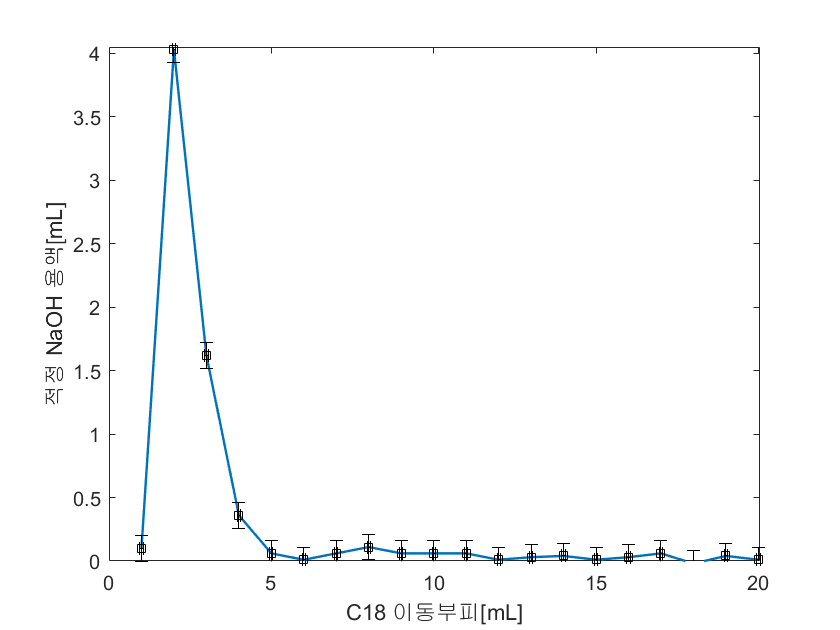
\includegraphics[width = 0.95\linewidth]{C18.png}% Here is how to import EPS art
	\caption{\label{fig:C18}크로마토그래피 후 적정 결과 그래프}
\end{figure}

\begin{table}[]
\begin{tabular}{c|c} \hline \hline
아세트산[$mmol$] & 살리실산 [$mmol$] \\ \hline
$6.2\pm0.1mmol$ & $2.6\pm0.1mmol$  \\ \hline \hline
\end{tabular}
\caption{\label{tab:NAOH_1}$M_{NaOH} = 1mM$인 경우}
\end{table}

\begin{table}[]
\begin{tabular}{c|c} \hline \hline
아세트산[$mmol$] & 살리실산 [$mmol$] \\ \hline
$25.5\pm0.3mmol$ & $10.9\pm0.1mmol$  \\ \hline \hline
\end{tabular}
\caption{\label{tab:NAOH_4}$M_{NaOH} = 4.14mM$인 경우}
\end{table}

\section{\label{sec:level1}Discussion}
$NaOH$의 표준화에서 $1mL$ 가 아닌 $0.1mL, 0.5mL$으로 표준화를 진행하였다. 시약의 부피를 측정하는 장비의 최소눈금으로 인해 발생하는 오차와 피펫에서 떨어뜨리는 적정용액의 최소부피로 인해 측정값과 오차사이의 상대비율이 증가하였고 결국 최종 실험결과에 큰 오차를 발생시켰을 것으로 예상한다. 한 부피에서만 적정하는 것이 아닌, $0.1 ... 0.9, 1.0mL$의 $KHP$용액을 적정하고 해당 값을 선형회귀하면 더 정확한 $NaOH$의 몰농도를 측정할 수 있을 것이다.

$NaOH$ 표준화에서 발생한 오차를 고려하여 이상적으로 농도가 $1.0mM$인 경우와 $4.14mM$인 경우를 분리하여 실험을 수행하였다. 그 결과 각각 $8.8mmol$, $36.4mmol$의 total acidity 가 측정되었다. 분리실험에서 이상적으로 모두 반응했을 경우 $8.8mL$가 반응했어야 했지만 $6.74mL$만이 반응하였다. 이것은 정지상과 결합한 살리실산이 완전히 배출되지 않아 발생한 것으로 결론지었다.

Fick's second law는 식(\ref{eq:fick})와 같다.[5] $D$는 확산계수로 물질과의 상호작용이 작아 빠르게 이동할수록 큰 값을 가진다. 따라서 본 실험에서 살리실산이 아세트산보다 작은 확산계수를 가짐을 알 수 있다. 해당식의 해는 (\ref{eq:sol})와 같다. 아세트산의 경우 빠르게 카트리지를 지나가므로 $Dt$값이 충분히 작아 sharp한 peak를 가진다. 반면에 살리실산은 $D$가 작음에도 불구하고 느리게 이동하여 $Dt$값이 커지게 되고 매우 broad한 peak를 가지게 된다.
\begin{align} 
	\frac{\partial n}{\partial t} &= D\frac{\partial^{2} n}{\partial x^{2}}\label{eq:fick}\\
	n(x,t) &= \frac{A}{\sqrt{Dt}}\exp\left(\frac{-x^{2}}{4Dt}\right)\label{eq:sol}
\end{align}

Normal phase chromatography를 이용하여 약산을 분리하는 경우 살리실산이 먼저 검출될 것이다.[1] 예를 들어 순수한 silica 혹은 amino를 정지상으로 사용하고 이동상으로 벤젠과 같은 무극성 분자들로 구성된 액체를 이용할 수 있다.[3] 또한 더 정확한 수치를 얻기 위해 HPLC를 이용해 각각의 물질의 농도를 측정할 수 있을 것이다.[1]



\section{\label{sec:level1}Reference}
[1] 김희준, \textit{일반화학 실험}(자유아카데미, 2016)\\

[2] D.W. Oxtoby, H.P. Gillis, and L. Butler, \textit{Principles of Modern Chemistry} (Brooks/Cole, Australia, 2020).

[3] D.C. Harris, \textit{Quantitative Chemical Analysis} (W.H. Freeman and Co., New York, 2010). 

[4] T.-J. Hsu, C.-C. Liao, and M.-Y. Chen, Journal of the Chinese Chemical Society 26, 21 (1979). 

[5] 1 C.J. Adkins and C.J. Adkins, \textit{An Introduction to Thermal Physics} (Cambridge University Press, Cambridge Cambridgeshire, 2004). 
\end{document}
%
% ****** End of file apssamp.tex ******
